\documentclass[addpoints,11pt,answers]{exam}
\usepackage[utf8]{inputenc}
\usepackage[english]{babel}
\usepackage{listings}
\usepackage{textcomp}
\usepackage{amsmath}
\usepackage{algpseudocode}
\usepackage{graphicx}
\usepackage{amssymb}
\usepackage{amsthm}
\usepackage{hyperref}
\usepackage{logicproof}
\usepackage{multicol}
\usepackage{environ}
\usepackage{xcolor}
 \usepackage{tikz}
\usetikzlibrary{arrows}
\usepackage{MnSymbol}

\tikzset{
  treenode/.style = {align=center, inner sep=0pt, text centered,
    font=\sffamily},
  nd_w/.style = {treenode, circle, black, draw=black, text width=1em, very thick},% node
  nd_filled/.style = {treenode, circle, black, draw=black, fill=gray, text width=1em, very thick},% node
  nd_b/.style = {treenode, circle, white, font=\sffamily\bfseries, draw=black,fill=black, text width=1em},% arbre rouge noir, noeud noir
  nd_r/.style = {treenode, circle, red, draw=red, text width=1em, very thick},% arbre rouge noir, noeud rouge
  nd_nil/.style = {treenode, rectangle, draw=black, fill=black, minimum width=0.5em, minimum height=0.5em}% null
}

\newcommand{\limit}[1]{ \lim_{n \rightarrow \infty} \left( #1 \right) }
\bracketedpoints
\qformat{Question \thequestion{} : \totalpoints{} \points \hfill}

%These setting will make the code areas look Pretty
\lstset{
	escapechar=~,
	numbers=left, 
	%numberstyle=\tiny, 
	stepnumber=1, 
	firstnumber=1,
	%numbersep=5pt,
	language=C,
	% stringstyle=\itfamily,
	%basicstyle=\footnotesize, 
	showstringspaces=false,
	frame=single,
  upquote=true
}

\title{CS260 - Data Structures \\ Written Assignment 5}
\author{Jonathan Parlett} 

\begin{document}
\maketitle

\begin{questions}
%%%%%%%%%%%%%%%%%%%%%%%%%%
%%%% Question 1 %%%%%%%%%%
%%%%%%%%%%%%%%%%%%%%%%%%%%
\question
Given an undirected graph $G=(V,E)$, two vertices $u,v \in V$ are called {\bf connected vertices} if there exist a path in $G$ from $u$ to $v$, and called disconnected otherwise.\\

The same graph $G$ is called a {\bf connected graph} if every vertex pair $u,v \in V$ is connected, indicating that there exists a path between any two vertices in the graph.\\

\begin{parts}
 \part[7] Suggest an algorithm in plain English that determines whether a given undirected graph is connected or disconnected.
 \begin{solution}
  Since the given graph is undirected is suffices to check if any one of the nodes can reach all the others. In this way we simply need to check if 
  every node is colored black after running BFS, or equivalently if the count of black nodes equals the count of total nodes. By keeping a running count
  of black nodes during the execution of BFS we ensure that the extra amount of work is constant.
 \end{solution}
 
 \part[4] Provide pseudocode of your algorithm.
  \begin{solution}
    \\
    After the below algorithm returns we simply need to check if (blackCount==$G\to size$)
  \begin{lstlisting}
int bfs(graph* G, vertex* s){

  if(s == NULL) return 0;

  //init queue
  queue* Q = Queue();

  int blackCount=0; //count of black nodes

  anode* c = s->alisthead;
  while(c != NULL){
    if(G->V[c->vertex]->color == 'w'){
      G->V[c->vertex]->color = 'g';
      enqueue(Q,G->V[c->vertex]);
    }
    c = c->next;
  }
  
  //blacken s were done with it
  s->color = 'b';
  blackCount++;
  //check all neighbors
  while(Q->size != 0)
    blackCount += bfs(G, dequeue(Q));

  free(Q);
  return blackCount;
} 
 \end{lstlisting}
 \end{solution}
 
 \part[4] What is the runtime of your algorithm? Show your analysis.
  \begin{solution}
  Runtime is $O(n+m)$ since the only extra work is just incrementing a counter.
 \end{solution}
 
\end{parts}

%%%%%%%%%%%%%%%%%%%%%%%%%%
%%%% Question 2 %%%%%%%%%%
%%%%%%%%%%%%%%%%%%%%%%%%%%
\question
You are given a weighted undirected graph $G=(V,E)$, where $E$ and $V$ denote set of edges and vertices, and a minimum spanning tree $T$ of that graph $G$. Answer the following questions about $G$ and $T$ on minimum spanning trees.
\begin{parts}
 \part[10] Suppose we decrease the weight of one of the edges in $G$ that is not among the edges in $T$. Suggest an algorithm in plain English that determines whether $T$ is still a minimum spanning tree, and if it is not, calculates a minimum spanning tree of $G$. Explain the running time of your algorithm. (Note: Your algorithm should be faster than Prim's and Kruskal's) 
  \begin{solution}
  \\
  If the new edge = $(u,v)$ we need to find the current edge $(u,v)$ in the tree and compare their weights. If the weight of the new is less than the current
    than  we remove the old from the edge set and add the new.
 \end{solution}
 
 \part[5] Consider the following algorithm running on $G=(V,E)$. Would it calculate a valid MST of $G$? If yes, explain your reasoning in plain English, if no, provide a counter example graph that the algorithm will fail producing an MST.
 
 \begin{lstlisting}[escapeinside={(*}{*)}]
MSTcandidate(G)
 E = sort G.E in inverse order of edge weights
 T = E
 for i from 1 to |E| do
    if T - {e} is a connected graph
        T = T - {e}
    end if
 end for
 return T
\end{lstlisting}
 \begin{solution}\\
  This algorithm seems to suggest we remove the most expensive edges, as long as it maintains the connected graph property, to create our MST.
   This guarantees that we will remove any edge that creates a cycle since we attempt to remove all edges. So yes this algorithm will produce a
   valid MST.
 
 \end{solution}
 
 \part[5] What is the running time of the algorithm in the previous question. Show your analysis.
 \begin{solution}\\
   Sorting all edges weights takes at least $O(ElogE)$ time. Checking for a connected graph takes $O(V+E)$ time and we will do this $E$ times in the for loop.
   So runtime would be $O(ElogE + E(V+E)) = O(ElogV + V^3 + V^4)$. So runtime would be $O(V^4)$.
 
 \end{solution}
 
 \end{parts}

\newpage 

%%%%%%%%%%%%%%%%%%%%%%%%%%
%%%% Question 3 %%%%%%%%%%
%%%%%%%%%%%%%%%%%%%%%%%%%%
\question After you graduate, you got hired by an IT consulting company that offers services to a wide spectrum of customers. You were assigned to a company called ACME Roadworks Inc. that is a contractor for building roads and infrastructure. They got a new job from the City of Philadelphia for updating the water pipes in Powelton Village. The job consists of connecting houses to each other which will then get connected to the city's main water pipe. Since water comes from a single source and flows towards houses, there should not be any cycle in the pipe system. Although the goal should be to build the pipe tree structure with minimum amount of pipes, the boss of the company Evelyn Deavor is asking you to come up with a structure that spans all houses with maximum length of pipes. Although this request deeply disturbed your conscience, you couldn't turn down the job as your roommate reminded you of your upcoming student loan payments... Then, answer the following questions:

\begin{parts}
\part[5] Formulate the task as a graph problem. What are the nodes? What are the edges? Is this a weighted graph? If so, what are the weights? Is the graph directed? What is the goal to achieve over this graph?
 \begin{solution}\\
   The nodes would be the houses and the cities main water pipe. The weights would be the length of pipes connecting locations. The graph need not be directed
   it suffices for it to be connected so that everything is reachable by the main pipe. The goal is the find the maximal spanning tree. The tree with the most
   expensive edges.
 \end{solution}
 
\part[5] Suggest an algorithm in plain English to solve the problem.
 \begin{solution}\\
  Let us start with the complete graph $K_v$ and assign waits by pipe length. Then negate all all edge weights so that the largest become the smallest in the
   ordered list of edges. Then we could use the algorithm from question 2 or prims or kruskals to generate the MST. After this we can simply negate all edges
   again to get our maximal spanning tree.
 \end{solution}
 
\part[5] Analyze the running time of your algorithm.
 \begin{solution}
  The only additional work is negating all edges weights twice. So we add $2E$ amount of work to any MST algorithm we choose to use. Since $2E$ is insignificant to
   the runtime of any MST algorithm. Runtime of is just the runimte of the algorithm chosen. Either $O(ElogV)$ or $O(V^4)$.
 \end{solution}
 
\end{parts}

%%%%%%%%%%%%%%%%%%%%%%%%%%
%%%% Question 4 %%%%%%%%%%
%%%%%%%%%%%%%%%%%%%%%%%%%%
\question [20]
Run Dijkstra's single source shortest path algorithm on the graph given below to calculate shortest path from $c$ to every other node. Draw the graph and the content of the priority queue for each iteration. First two steps are provided below as an example for you. When answering the question, either use the provided answers to copy/paste the \LaTeX ~code for producing the rest of the figures, or draw your answer over a paper and include it inside the document as an image. (Note: You can show the contents of the heap as a sorted array, don't worry about writing the heap as how it should be in memory.)

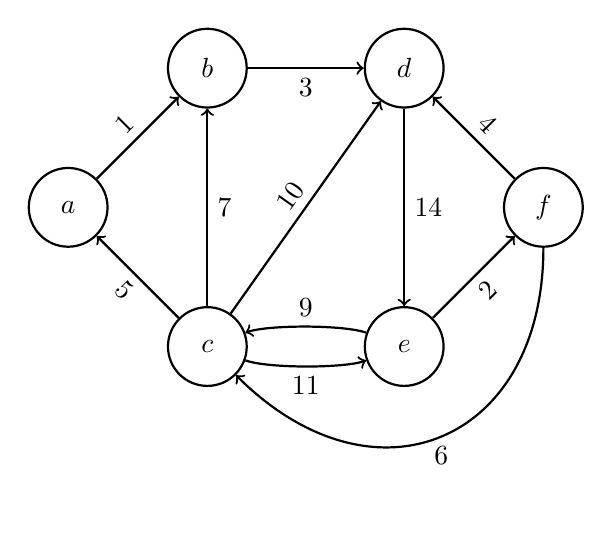
\begin{tikzpicture}[node distance={25mm}, thick, main/.style = {draw, circle,minimum size=10mm}] 
\node[main] (a) {$a$}; 
\node[main] (b) [above right of=a] {$b$}; 
\node[main] (c) [below right of=a] {$c$}; 
\node[main] (d) [right of=b] {$d$}; 
\node[main] (e) [right of=c] {$e$}; 
\node[main] (f) [below right of=d] {$f$}; 
\draw[->] (a) -- node[above,sloped] {1} (b); 
\draw[->] (b) -- node[below] {3} (d); 
\draw[->] (c) -- node[right] {7} (b);
\draw[->] (c) -- node[below,sloped] {5} (a); 
\draw[->] (c) -- node[above,sloped] {10} (d); 
\draw[->] (c) to [out=-20,in=-160,looseness=0.5] node[below] {11} (e);
\draw[->] (e) to [out=160,in=20,looseness=0.5] node[above] {9} (c);
\draw[->] (e) -- node[below,sloped] {2} (f); 
\draw[->] (f) -- node[above,sloped] {4} (d); 
\draw[->] (f) to [out=-90,in=-45,looseness=1.5] node[below] {6} (c);
\draw[->] (d) -- node[right] {14} (e); 
\end{tikzpicture} 

 {\bf Iteration 0:} Distance of every other node to $c$ is set to $\infty$, distance of $c$ to itself is set to 0, $c$ is inserted into the heap, and will be extracted in the next iteration as it is the minimum in the heap.\\
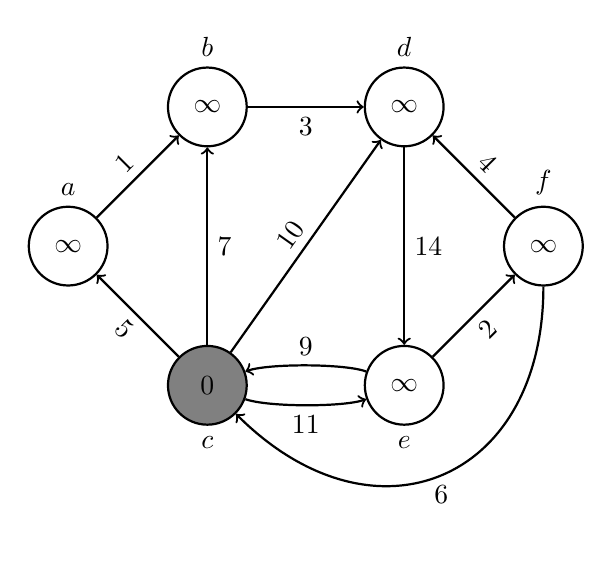
\begin{tikzpicture}[node distance={25mm}, thick, main/.style = {draw, circle,minimum size=10mm}] 
\node[main] (a) [label=above:{$a$}]{$\infty$}; 
\node[main] (b) [above right of=a,label=above:{$b$}] {$\infty$}; 
\node[main] (c) [below right of=a,label=below:{$c$},fill=gray] {$0$}; 
\node[main] (d) [right of=b,label=above:{$d$}] {$\infty$}; 
\node[main] (e) [right of=c,label=below:{$e$}] {$\infty$}; 
\node[main] (f) [below right of=d,label=above:{$f$}] {$\infty$}; 
\draw[->] (a) -- node[above,sloped] {1} (b); 
\draw[->] (b) -- node[below] {3} (d); 
\draw[->] (c) -- node[right] {7} (b);
\draw[->] (c) -- node[below,sloped] {5} (a); 
\draw[->] (c) -- node[above,sloped] {10} (d); 
\draw[->] (c) to [out=-20,in=-160,looseness=0.5] node[below] {11} (e);
\draw[->] (e) to [out=160,in=20,looseness=0.5] node[above] {9} (c);
\draw[->] (e) -- node[below,sloped] {2} (f); 
\draw[->] (f) -- node[above,sloped] {4} (d); 
\draw[->] (f) to [out=-90,in=-45,looseness=1.5] node[below] {6} (c);
\draw[->] (d) -- node[right] {14} (e); 
\end{tikzpicture} 

 $Q=$
 \begin{tabular}{|c|c|c|c|}
    \hline
    $c$ &  &  &  \\
    \hline
\end{tabular}\\

{\bf Iteration 1:} Once $c$ is extracted from the heap, edges $(c,a), (c,b), (c,d),$ and $(c,e)$ are relaxed, updating the distances of nodes $a,b,d,e$ to 5,7,10,11 respectively. These edges are highlighted as they take their respective nodes to theor parent node $c$ in the current shortest path three. Nodes $a,b,d,e$ are inserted into the heap. Since $a$ is the min in the heap, it will get extracted at the beginning of the next iteration (hence highlighted in grey)\\
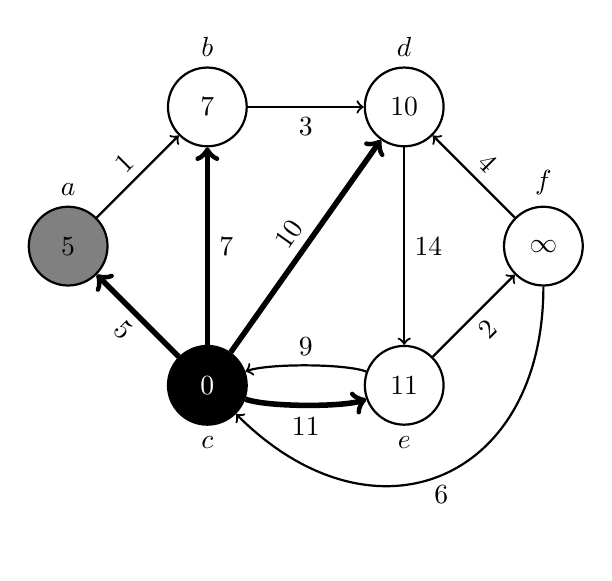
\begin{tikzpicture}[node distance={25mm}, thick, main/.style = {draw, circle,minimum size=10mm}] 
\node[main] (a) [label=above:{$a$},fill=gray]{$5$}; 
\node[main] (b) [above right of=a,label=above:{$b$}] {$7$}; 
\node[main] (c) [below right of=a,label=below:{$c$},fill=black,text=white] {$0$}; 
\node[main] (d) [right of=b,label=above:{$d$}] {$10$}; 
\node[main] (e) [right of=c,label=below:{$e$}] {$11$}; 
\node[main] (f) [below right of=d,label=above:{$f$}] {$\infty$}; 
\draw[->] (a) -- node[above,sloped] {1} (b); 
\draw[->] (b) -- node[below] {3} (d); 
\draw[->,line width=2pt] (c) -- node[right] {7} (b);
\draw[->,line width=2pt] (c) -- node[below,sloped] {5} (a); 
\draw[->,line width=2pt] (c) -- node[above,sloped] {10} (d); 
\draw[->,line width=2pt] (c) to [out=-20,in=-160,looseness=0.5] node[below] {11} (e);
\draw[->] (e) to [out=160,in=20,looseness=0.5] node[above] {9} (c);
\draw[->] (e) -- node[below,sloped] {2} (f); 
\draw[->] (f) -- node[above,sloped] {4} (d); 
\draw[->] (f) to [out=-90,in=-45,looseness=1.5] node[below] {6} (c);
\draw[->] (d) -- node[right] {14} (e); 
\end{tikzpicture} 

 $Q=$
 \begin{tabular}{|c|c|c|c|}
    \hline
    $a$ & $b$ & $d$ & $e$ \\
    \hline
\end{tabular}\\

{\bf Iteration 2:} $a$ is extracted from the heap. The only node in its adjacency list $b$ is checked to see if the edge relaxes, which it does. The distance of $b$ is relaxed to become 6, rather than 7. The parent pointer of $b$ is changed to become $a$ rather than $c$ due to this relaxation. Edge $(a,b)$ is highlighted accordingly, replacing $(c,d)$. Being the smallest distance in the heap, node $b$ will be extracted in the next iteration.\\
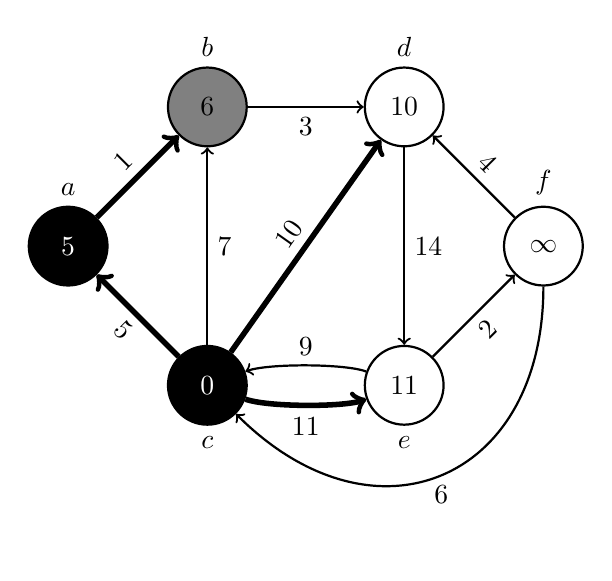
\begin{tikzpicture}[node distance={25mm}, thick, main/.style = {draw, circle,minimum size=10mm}] 
\node[main] (a) [label=above:{$a$},fill=black,text=white]{$5$}; 
\node[main] (b) [above right of=a,label=above:{$b$},fill=gray] {$6$}; 
\node[main] (c) [below right of=a,label=below:{$c$},fill=black,text=white] {$0$}; 
\node[main] (d) [right of=b,label=above:{$d$}] {$10$}; 
\node[main] (e) [right of=c,label=below:{$e$}] {$11$}; 
\node[main] (f) [below right of=d,label=above:{$f$}] {$\infty$}; 
\draw[->,line width=2pt] (a) -- node[above,sloped] {1} (b); 
\draw[->] (b) -- node[below] {3} (d); 
\draw[->] (c) -- node[right] {7} (b);
\draw[->,line width=2pt] (c) -- node[below,sloped] {5} (a); 
\draw[->,line width=2pt] (c) -- node[above,sloped] {10} (d); 
\draw[->,line width=2pt] (c) to [out=-20,in=-160,looseness=0.5] node[below] {11} (e);
\draw[->] (e) to [out=160,in=20,looseness=0.5] node[above] {9} (c);
\draw[->] (e) -- node[below,sloped] {2} (f); 
\draw[->] (f) -- node[above,sloped] {4} (d); 
\draw[->] (f) to [out=-90,in=-45,looseness=1.5] node[below] {6} (c);
\draw[->] (d) -- node[right] {14} (e); 
\end{tikzpicture} 

 $Q=$
 \begin{tabular}{|c|c|c|c|}
    \hline
    $b$ & $d$ & $e$ &  \\
    \hline
\end{tabular}\\

 \begin{solution}
   The paths in blue represent the arcs taken on each shortest path through the graph.
   \includegraphics{IMG_1030.jpg}
   \includegraphics{IMG_1032.jpg}
 \end{solution}
 

%%%%%%%%%%%%%%%%%%%%%%%%%%
%%%% Question 5 %%%%%%%%%%
%%%%%%%%%%%%%%%%%%%%%%%%%%
\question [15] Run Floyd-Warshall all pairs shortest path algorithm on the graph below. Show the distance matrix $D^{(k)}$ for each iteration $k$. 

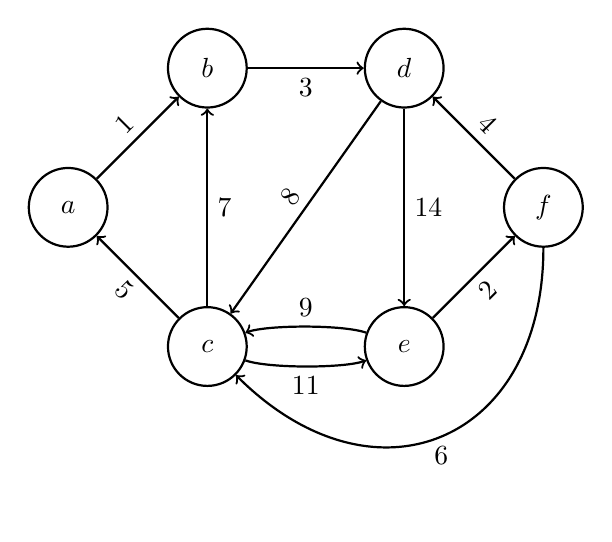
\begin{tikzpicture}[node distance={25mm}, thick, main/.style = {draw, circle,minimum size=10mm}] 
\node[main] (a) {$a$}; 
\node[main] (b) [above right of=a] {$b$}; 
\node[main] (c) [below right of=a] {$c$}; 
\node[main] (d) [right of=b] {$d$}; 
\node[main] (e) [right of=c] {$e$}; 
\node[main] (f) [below right of=d] {$f$}; 
\draw[->] (a) -- node[above,sloped] {1} (b); 
\draw[->] (b) -- node[below] {3} (d); 
\draw[->] (c) -- node[right] {7} (b);
\draw[->] (c) -- node[below,sloped] {5} (a); 
\draw[->] (c) to [out=-20,in=-160,looseness=0.5] node[below] {11} (e);
\draw[->] (d) -- node[above,sloped] {8} (c); 
\draw[->] (d) -- node[right] {14} (e); 
\draw[->] (e) to [out=160,in=20,looseness=0.5] node[above] {9} (c);
\draw[->] (e) -- node[below,sloped] {2} (f); 
\draw[->] (f) -- node[above,sloped] {4} (d); 
\draw[->] (f) to [out=-90,in=-45,looseness=1.5] node[below] {6} (c);

\end{tikzpicture} 

The matrix for the first two iterations (i.e., $D^{(0)}$ and $D^{(1)}$ are shown below as a reference where rows and columns represent nodes in alphabetical order. You need to show matrices up to $D^{(5)}$.

{\bf Iteration 0:} Initialize direct connections with the weight of edges, set self edges to zero, and set everything else to $\infty$. \\
$D^{(0)}=\begin{bmatrix}
 0 & 1 & \infty & \infty & \infty & \infty \\
 \infty & 0 & \infty & 3 & \infty & \infty \\
 5 & 7 & 0 & \infty & 11 & \infty \\
 \infty & \infty & 8 & 0 & 14 & \infty \\
 \infty & \infty & 9 & \infty & 0 & 2 \\
 \infty & \infty & 6 & 4 & \infty & 0 
\end{bmatrix}$\\

{\bf Iteration 1:} $D^{(1)}$ represents the shortest path between any two nodes $u$ and $v$, by using only the first node (that is node $a$) as an intermediary node on the shortest path. By adding $a$ to possible intermediary nodes, only the path between $c$ and $b$ gets shorter. The rest of the matrix do not change. \\
$D^{(1)}=\begin{bmatrix}
 0 & 1 & \infty & \infty & \infty & \infty \\
 \infty & 0 & \infty & 3 & \infty & \infty \\
 5 & 6 & 0 & 8 & 11 & \infty \\
 \infty & \infty & \infty & 0 & 14 & \infty \\
 \infty & \infty & 9 & \infty & 0 & 2 \\
 \infty & \infty & 6 & 4 & \infty & 0 
\end{bmatrix}$\\

 \begin{solution}
   {\bf Iteration 2:} $D^{(2)}$ Next we add $b$ to the set of internal nodes and adjust weights accordingly.
   Now $a$ and $c$ can reach $d$ so we can updates the distance.
 $D^{(2)}=\begin{bmatrix}
   0 & 1 \\
   \infty & 0\\
   5 & \\
   \infty\\
   \infty\\
   \infty\\
\end{bmatrix}$\\

  
 
 \end{solution}
 

%%%%%%%%%%%%%%%%%%%%%%%%%%
%%%% Question 6 %%%%%%%%%%
%%%%%%%%%%%%%%%%%%%%%%%%%%
\question
In economics, arbitrage is the practice of taking advantage of a difference in prices in two or more markets; striking a combination of matching deals to capitalize on the difference, the profit being the difference between the market prices at which the unit is traded.\\

Arbitrage can become a source of gain when applied to currency exchanges. Consider the following currency exchange ratios as an example: 1 U.S. dollar buys 0.7292 euros, 
1 euro buys 105.374 Japanese yen, 1 Japanese yen buys 0.3931 Russian rubles, 1 Russian ruble buys 0.0341 U.S. dollars.\\

Then you could take 1 U.S. dollar and buy 0.7292 euros with it, with which you can buy 76.8387 yen (because 0.7292 * 105.374 = 76.8387). Then take the 76.8387 yen and buy 30.2053 rubles (because 76.8387 * 0.3931 = 30.2053), and finally take the 30.2053 rubles and buy 1.03 dollars (because 30.2053 * 0.0341 = 1.0300). \\

Assume that you are given the pairwise trading ratios among $n$ currencies and answer the following questions about arbitrage accordingly.

\begin{parts}
\part[5] Formulate the task as a graph problem. What are the nodes? What are the edges? Is this a weighted graph? If so, what are the weights? Is the graph directed? What is the goal to achieve over this graph?
 \begin{solution}
  The graph would be weighted and directed. The nodes in this case would be the currencies and the edge weights would be the trading ratios
  between currencies.
 \end{solution}
 
\part[5] Suggest an algorithm in plain English that evaluate whether an arbitrage exists among these $n$ currencies.
 \begin{solution}
  An arbitrage exists if there is a cycle such that the product of the edge costs is greater than 1. This can be seen in the procided example.
   We can find such a cycle by changing the problem into an equivalent one.
  \begin{itemize}
    \item take the logarithm of all edge weights (since the log of a product is the sum of the logs)
    \item negate all edge weights, in this way we have transformed the goal into finding a negative weight cycle
    \item run-bellman ford to compute all shortest paths from a node of weight 0 connected to the graph
    \item for all edges with a negative weight $(u,v)$ check if tracing the predecessors of $u$ leads back to $u$
  \end{itemize}
   If the last steps succeeds in finding such a node then we have found a negative weight cycle that we can exploit for arbitrage.
 \end{solution}
 
\part[5] Analyze the running time of your algorithm.
 \begin{solution}
  We must take the log of and negate all egde weights which is linear in number of edges $O(E)$. Bellman-Ford is a $O(v^3)$
   and then finding a negative weight cycle takes another $O(E+V)$ since potentially the cycle constitutes the entire graph.
   So runtime is $O(E+E+V+V^3)=O(V^3)$.
 \end{solution}
 
\end{parts}

\end{questions}
\end{document}
